\section{Durchführung}
\label{sec:Durchführung}
\subsection{Versuchsaufbau}
\label{sec:aufbau}
Der Versuchsaufbau besteht aus einer Transparenten Platte auf welcher sich ein roter
($\lambda=\SI{635}{\nano\metre}$) und ein grüner ($\lambda=\SI{532}{\nano\metre}$) Laser 
befinden. Die Laser lassen sich dabei im Halbkreis um die Platte bewegen, sodass verschiedene
Winkel eingestellt werden können. Diese können dann an der Skala auf der Platte abgelesen werden.
Um die Experimentierenden vor dem Laserlicht zu schützen ist zudem noch ein Reflexionsschirm
verbaut. Diese Apparatur ist in Abbildung \ref{fig:Aufbau} dargestellt.
\\\noindent 
In der Mitte der Apparatur \ref{fig:Aufbau} lassen sich nun optische Elemente positionieren, welche
in Abbildung \ref{fig:Teile} dargestellt sind. 
\begin{figure}[H]
    \centering
    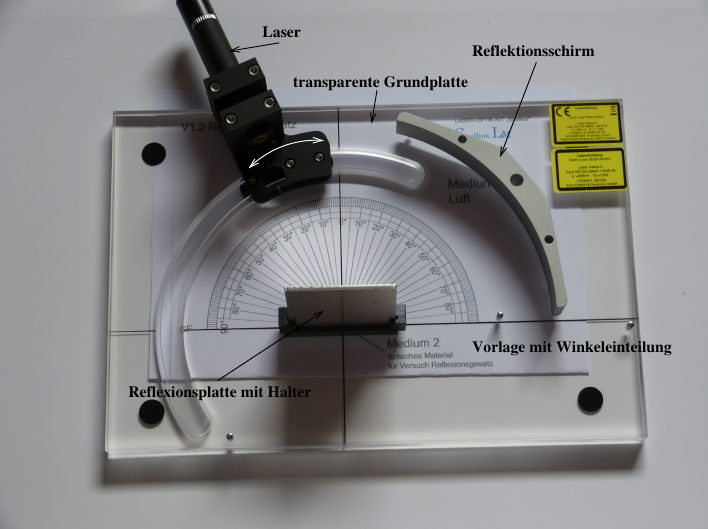
\includegraphics[scale = 0.3]{pictures/Aufbau.png}
    \caption{Die Versuchsapparatur. Quelle: \cite{AP01}}
    \label{fig:Aufbau}
\end{figure}
\begin{figure}[H]
    \centering
    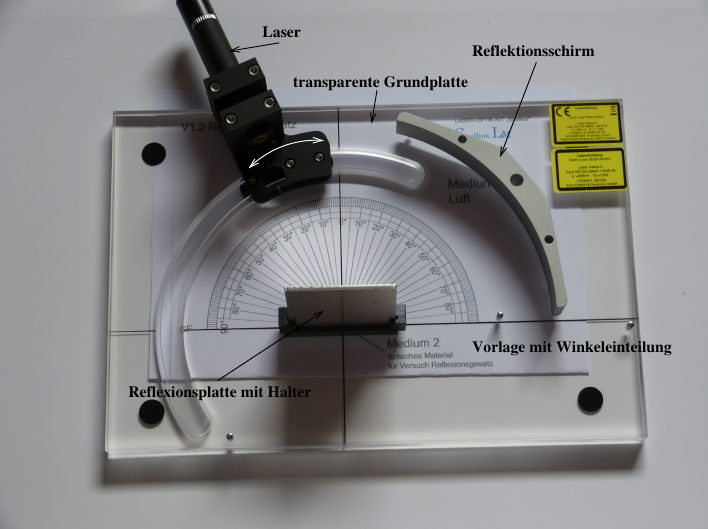
\includegraphics[scale = 0.3]{pictures/Teile.png}
    \caption{Optische Elemente. Quelle: \cite{AP01}}
    \label{fig:Teile}
\end{figure}

\subsection{Reflexionsgesetz}
\label{sec:reflexionsmessung}
\subsection{Brechungsgestz}
\label{sec:brechungmessung}
\section{Strahlenversatz}
\label{sec:strahlenversatzmessung}
\section{Prisma}
\label{sec:prismamessung}